\documentclass{article}
\usepackage[export]{adjustbox}
\usepackage{graphicx}
\usepackage{fancyvrb}
\usepackage{booktabs}

\title{Reporte Actividad 6}
\author{Andr\'es Rodr\'iguez}
\date{}


\begin{document}

\maketitle

\graphicspath{ {Imagenes/} }



\section{Introducci\'on}
Se realiza un programa que ejecuta una simulaci\'on del movimiento de un proyectil, ahora considerando los efectos de fricci\'on causados por arrastre del aire. La simulaci\'on se realiza para el caso de una bola esf\'erica.

Durante la ejecuci\'on del programa se requiere ingresar la densidad del fluido en que se realiza el movimiento y las propiedades relevantes del objeto lanzado (radio, masa). Adem\'as, se ingresa el \'angulo de inicial, magnitud de velocidad incial, y la posici\'on inicial en $x$ y $y$.

El programa realiza los c\'alculos correspondientes a la trayectoria considerando la fuerza de arrastre causada, y en el caso de despreciarla. Los datos de estos dos c\'alculos se guardan cada uno en un archivo .dat, los cuales se utilizan para comparar los resultados y graficar. \\

\section{Marco te\'orico}
Usualmente se asume que los efectos de la resistencia del aire son despreciables. Cuando se omite la resistencia del aire, la \'unica fuerza actuando sobre un proyectil de masa $m$   es igual a su peso, por lo que la componente de la aceleraci\'on en el eje $X$ es cero.

Sin embargo, la resistencia del aire (fuerza de arrastre) tiene un mayor efecto sobre el movimiento de diversos objetos.  Cuado \'esta se incluye en el c\'alculo, la fuerza de arrastre es aproximadamente proporcional al cuadrado de la rapid\'ez relativa del proyectil respecto al aire:
$$f=Dv^2,$$
donde $D$ es una constante que depende de la densidad del aire $\rho$, el coeficiente de arrastre del proyectil $C$ y su secci\'on transversal $A$ del objeto
$$D=\frac{\rho C A}{2}.$$
Para bolas esfericas el valor del coeficiente de arrastre es $C \approx 0.47$. Ahora, considerando la fuerza causada por la resistencia del aire y la gravedad, los componentes de la aceleraci\'on del proyectil son:
$$a_x=-(D/m)vv_x, \qquad a_y=-g-(D/m)vv_y,$$.
Debido a esto, la velocidad en $x$ tampoco es constante. Las componentes de la velocidad a cada instante de tiempo son
$$v_x + \Delta v_x = v_x + a_x \Delta t, \qquad 
v_y + \Delta v_y = v_y + a_y \Delta t,$$

y finalmente, las coordenadas en cada instante de tiempo se calculan con las ecuaciones
$$x + \Delta x = x + v_x \Delta t + \frac{1}{2} a_x (\Delta t)^2, \quad y + \Delta y = y + v_y \Delta t + \frac{1}{2} a_y (\Delta t)^2.$$


\section{Resultados}
Como resultado del programa, se muestra en la imagen que sigue un ejemplo de la toma de pantalla de la ejecuci\'on para generar los datos:\\
\begin{center}
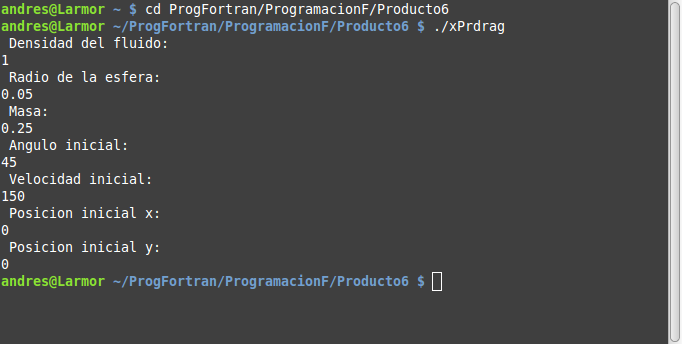
\includegraphics[scale=.5]{ej}\\
\end{center}

\subsection*{Diferencias en la distancia m\'axima recorrida:}
N\'otese que en todos los casos el fluido en que se desplaza el objeto es el aire, donde se toma $\rho \approx 1$. Y se defini\'o arbitrariamente los siguentes valores iniciales:\\ \\
$v_0 = 150 \: m/s, \quad x_0 = 0 \: m, \quad y_0 = 0 \: m.$\\
\begin{table}[h]
\caption {Diferencia en distancia m\'axima} \label{tab:title}
\begin{center}
\begin{tabular}{@{}lll|l@{}}
\toprule
     & Con arrastre & Sin arrastre & Diferencia \\ \midrule
$60 ^{\circ}$ & 246.97 m     & 1980.00 m    & 1733.03 m  \\
$45 ^{\circ}$  & 281.11 m     & 2291.03 m    & 2009.92 m  \\
$30 ^{\circ}$  & 292.07 m     & 1974.54 m    & 1682.47 m  \\ \bottomrule
\end{tabular}
\end{center}
\end{table}

\section{Gr\'aficas}
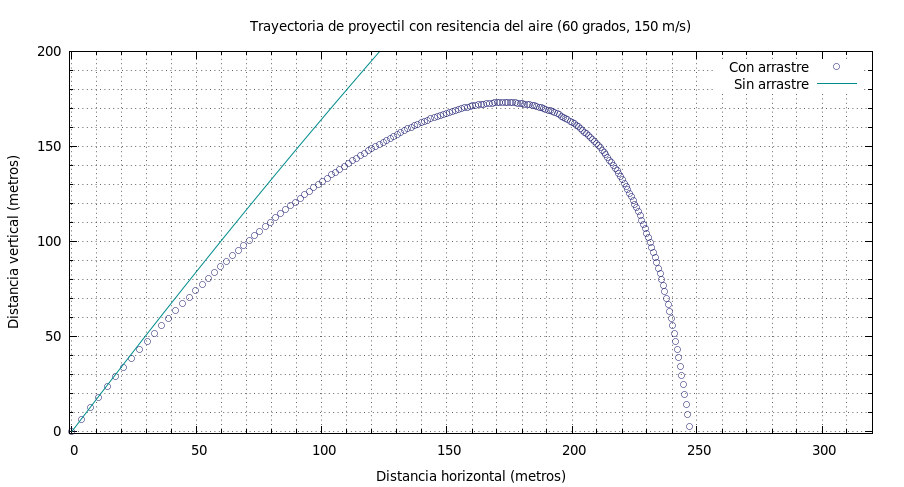
\includegraphics[scale=.5]{d60}\\
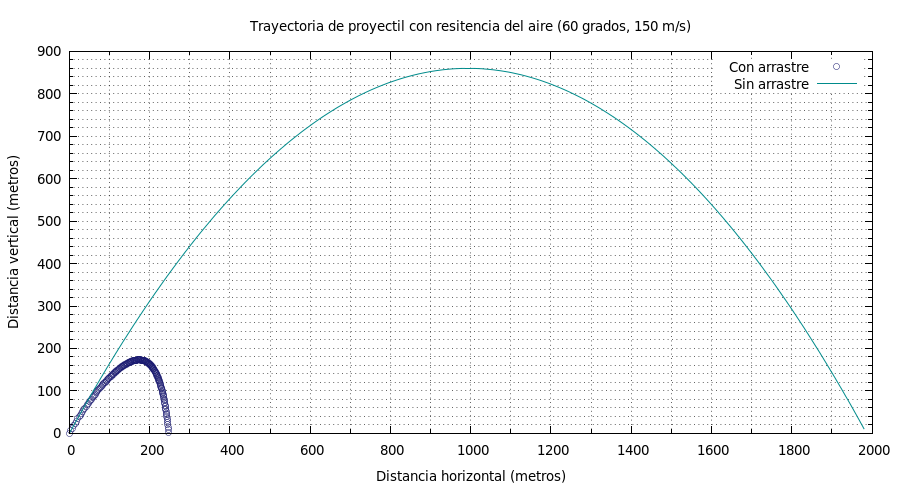
\includegraphics[scale=.5]{nd60}\\
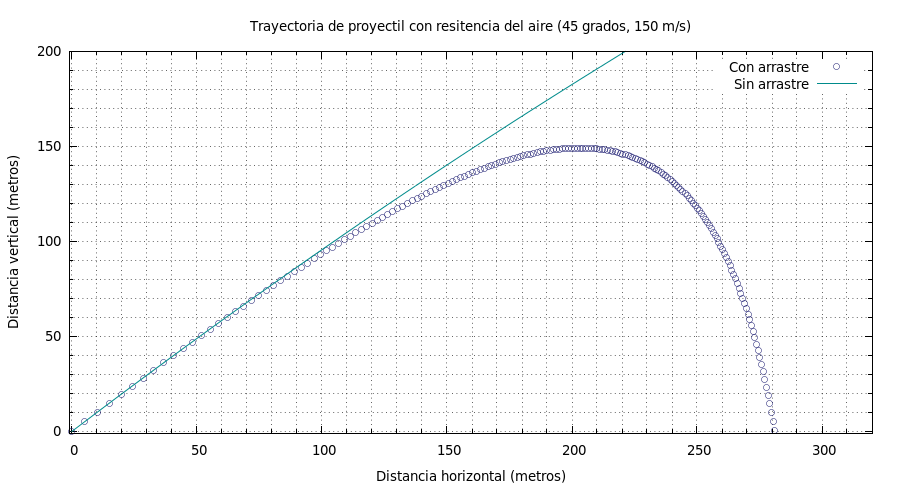
\includegraphics[scale=.5]{d45}\\
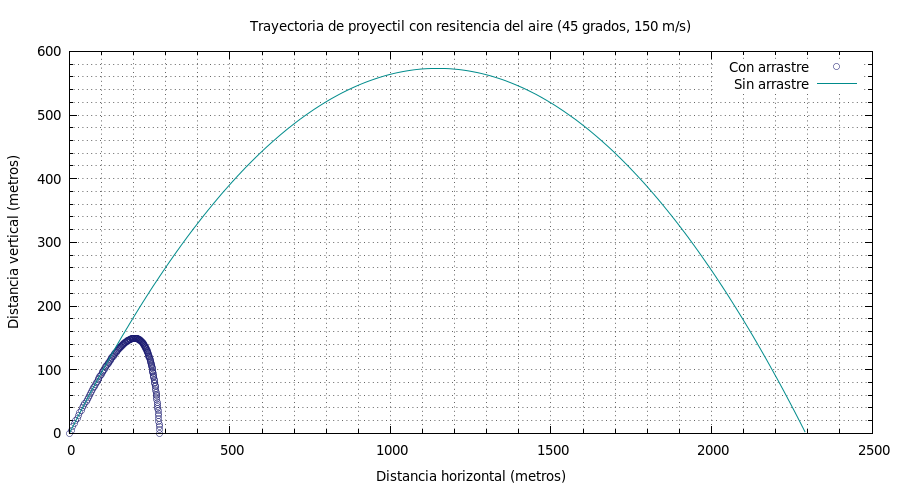
\includegraphics[scale=.5]{nd45}\\
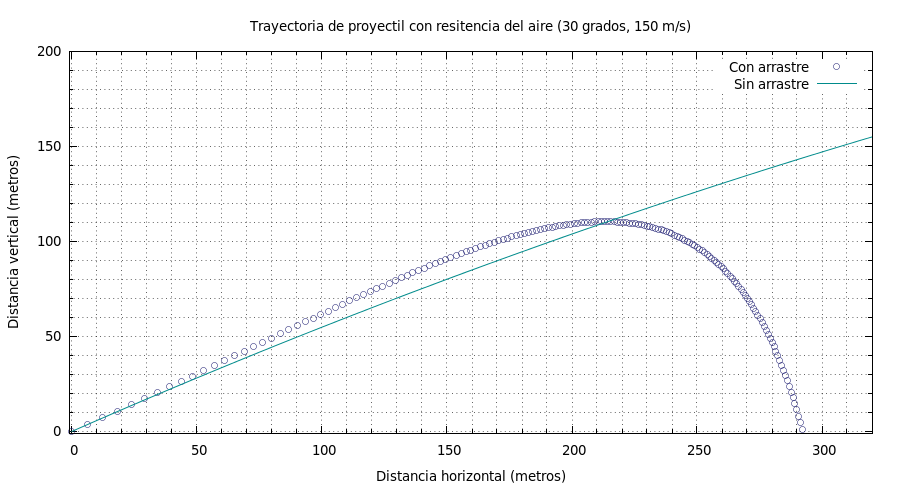
\includegraphics[scale=.5]{d30}\\
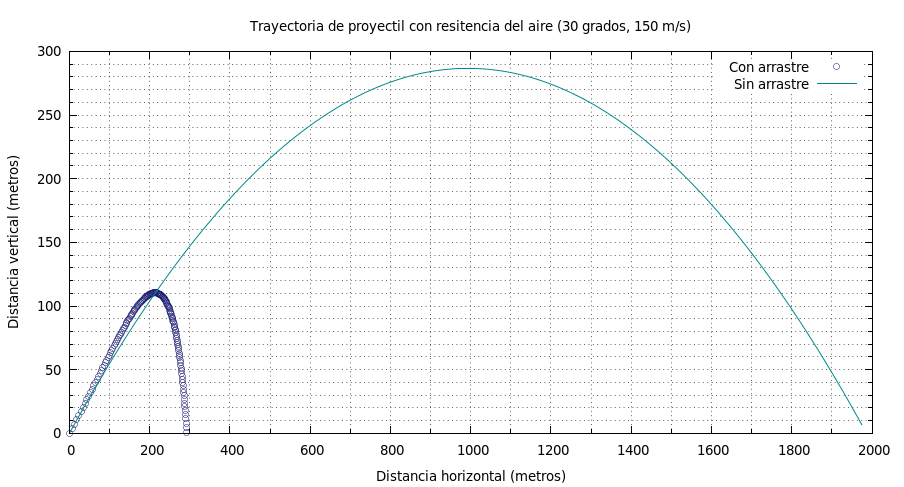
\includegraphics[scale=.5]{nd30}\\

\section{C\'odigo}\

C\'odigo Fortran:
\begin{Verbatim}[frame=single]

program projectile_plot  
       implicit none  

! DECLARACION DE VARIABLES
       real :: u, a, t_max, a_grados, D, rho, C, At
       real :: x0, y0, vx0, vy0,  ax, ay, m,r
       real :: xi,xii,yi,yii,yi2
       real :: x(1000),y(1000)  
          integer :: i = 0
          real :: t=0, dt=0.05


! DECLARACION DE CONSTANTES
       real, parameter :: pi = 4.0*atan(1.0) 
       real, parameter :: g = 9.81

       write(*,*) 'Densidad del fluido: '
       read *, rho
       write(*,*) 'Radio de la esfera: '
       read *, r
       write(*,*) 'Masa:'   
       read *, m

       C=0.47
       At= pi*r*r
       D = rho*C*At/2.0
     

       write(*,*) 'Angulo inicial:'   
       read *, a_grados   
       write(*,*) 'Velocidad inicial:'   
       read *, u   
       write(*,*) 'Posicion inicial x:'   
       read *, x0   
       write(*,*) 'Posicion inicial y:'   
       read *, y0
 

!CONVERTIR ANGULO A RADIANES 
       a = a_grados*pi/180.0   
       
!COMPONENTES DE VELOCIDAD
       vx0 = u*cos(a)
       vy0 = u*sin(a)

!!!!
       t_max= 2000*dt
       xi=x0
       yi=y0

!ABRIR ARCHIVO .DAT
       open(1, file='drag.dat')   
 
!CALCULO DE LA TRAYECTORIA CON RESISTENCIA DEL AIRE        
       do              
            call  FUERZA(g,D,m,vx0,vy0,ax,ay)
            call  TRAYECT(xi,yi,vx0,vy0,ax,ay,dt,xii,yii)
             if (yi<0) then
               exit
            end if
!ESCRIBIR CON FORMATO
            write(1,1000) xi, yi
            1000 format (2f8.2)
!REDEFINIR VARIABLES
            vx0 = vx0 + ax*dt
            vy0 = vy0 + ay*dt
            xi=xii
            yi=yii
       end do   
       close(1)


!CALCULO DE LA TRAYECTORIA SIN RESISTENCIA DEL AIRE
!(SE CONSIDERA D=0 Y SE TOMAN VALORES INICIALES x(0), y(0), u)
       
       vx0 = u*cos(a)
       vy0 = u*sin(a)
       xi=x0
       yi2=y0
       dt=0.1

       open(1, file='nodrag.dat')   
 
       do              
            call  FUERZA(g,0.0,m,vx0,vy0,ax,ay)
            call  TRAYECT(xi,yi2,vx0,vy0,ax,ay,dt,xii,yii)

             if (yi2 < 0 ) then
               exit
            end if
!ESCRIBIR CON FORMATO
            write(1,1001) xi, yi2
		1001 format (2f8.2)
!REDEFINIR VARIABLES
            vx0 = vx0 + ax*dt
            vy0 = vy0 + ay*dt
            xi=xii
            yi2=yii
       end do   
       
       close(1)

       

  
end program projectile_plot 


! SUBRUTINA CALCULO DE TRAYECTORIA

Subroutine TRAYECT(x1,y1,vx,vy,axi,ayi,dti,x2,y2)
Implicit None
real :: x1,y1,vx,vy,axi,ayi,dti,x2,y2

x2= x1 + vx*dti + 0.5*axi*dti*dti

y2= y1 + vy*dti + 0.5*ayi*dti*dti

End Subroutine TRAYECT


! SUBRUTINA CALCULO DE FUERZA DE ARRASTRE

Subroutine FUERZA(g,Di,mi,vx,vy,axi,ayi)
Implicit None
real :: g,Di,mi,vx,vy,axi,ayi

 axi = -(Di/mi) * vx * vx
 ayi = -g - (Di/mi)*vy*vy

End Subroutine FUERZA

\end{Verbatim}

\section{Referencia}

Proyectile Motion with Air Resistance,\\ http://wps.aw.com/wps/media/objects/877/898586/topics/topic01.pdf
\end{document}